% feedforward_velocidad.tex — explicación del feedforward de velocidad (IEE2913, Grupo 9), 17-11-2026
% Compilar con XeLaTeX (dos pasadas):  xelatex feedforward_velocidad.tex
% Las figuras se generan con docs/figuras/figuras_feedforward.py
\documentclass[11pt,a4paper]{article}
\usepackage[a4paper,margin=2.3cm,top=2.2cm,bottom=2.4cm]{geometry}
\usepackage{fontspec}
\usepackage{polyglossia}
\setdefaultlanguage{spanish}
\gappto\captionsspanish{\renewcommand{\tablename}{Tabla}}
\setmonofont{DejaVu Sans Mono}[Scale=0.80]
\usepackage{amsmath,amssymb}
\usepackage{graphicx}
\usepackage{booktabs,array,tabularx}
\usepackage{xcolor}
\usepackage{enumitem}
\usepackage{fancyvrb}
\usepackage{caption}
\usepackage{float}
\usepackage{titlesec}
\usepackage{fancyhdr}
\usepackage{tikz}
\usetikzlibrary{positioning,arrows.meta}
\usepackage[most]{tcolorbox}
\usepackage[hidelinks]{hyperref}

\graphicspath{{figuras/}}

\definecolor{tinta}{HTML}{0B0B0B}
\definecolor{tintados}{HTML}{52514E}
\definecolor{tenue}{HTML}{898781}
\definecolor{azul}{HTML}{2A78D6}
\definecolor{azulosc}{HTML}{184F95}
\definecolor{naranja}{HTML}{EB6834}
\definecolor{fondo}{HTML}{F4F7FC}
\definecolor{fondogris}{HTML}{F6F5F2}
\definecolor{regla}{HTML}{C3C2B7}

\color{tinta}
\setlength{\parindent}{0pt}
\setlength{\parskip}{0.55em}
\emergencystretch=2em
\setlist{itemsep=0.2em,topsep=0.25em,parsep=0.1em,leftmargin=1.5em}
\captionsetup{font=small,labelfont=bf,labelsep=period,skip=5pt}
\titleformat{\section}{\Large\bfseries\color{azulosc}}{\thesection.}{0.5em}{}
\titleformat{\subsection}{\large\bfseries}{\thesubsection}{0.5em}{}
\titlespacing*{\section}{0pt}{1.4em}{0.5em}
\titlespacing*{\subsection}{0pt}{1.0em}{0.3em}
\pagestyle{fancy}
\fancyhf{}
\renewcommand{\headrulewidth}{0pt}
\fancyfoot[L]{\small\color{tenue}IEE2913 · Grupo 9 · Feedforward de velocidad}
\fancyfoot[R]{\small\color{tenue}\thepage}

\newcommand{\cod}[1]{\texttt{#1}}
\newcommand{\lam}{\lambda}
\newcommand{\gr}{^{\circ}}
\newtcolorbox{clave}[1][]{enhanced,breakable,colback=fondo,colframe=azul,boxrule=0pt,leftrule=3pt,
  arc=0pt,left=9pt,right=9pt,top=6pt,bottom=6pt,before skip=0.8em,after skip=0.8em,fonttitle=\bfseries,
  coltitle=azulosc,colbacktitle=fondo,titlerule=0pt,attach title to upper={\par\smallskip},#1}
\newtcolorbox{lamina}[1]{enhanced,colback=white,colframe=regla,boxrule=0.6pt,arc=3pt,left=10pt,right=10pt,
  top=5pt,bottom=5pt,before skip=0.45em,after skip=0.45em,fonttitle=\bfseries,coltitle=azulosc,
  colbacktitle=white,titlerule=0pt,attach title to upper={\par\smallskip},title={#1}}
\DefineVerbatimEnvironment{codigo}{Verbatim}{fontsize=\small,frame=leftline,framerule=1.2pt,
  rulecolor=\color{regla},framesep=8pt,xleftmargin=4pt,baselinestretch=1.02}

\begin{document}

{\color{azulosc}\rule{\linewidth}{1.4pt}}

\vspace{0.5em}
{\LARGE\bfseries Feedforward de velocidad}\\[0.35em]
{\large Qué es, cómo está implementado en la RPi y en el ESP32, y cómo probarlo}\\[0.5em]
{\small\color{tintados}IEE2913 Diseño Eléctrico (Capstone) · Grupo 9 · Plataforma pan-tilt \hfill 17-11-2026}

\vspace{0.2em}
{\color{regla}\rule{\linewidth}{0.5pt}}

\begin{clave}[title={Lo esencial}]
\begin{itemize}[leftmargin=1.2em]
  \item \textbf{Qué es.} Además de decirle al ESP32 \emph{dónde} apuntar ($\theta_{\mathrm{ref}}$), la RPi le dice
        \emph{a qué velocidad} se mueve el objetivo ($\omega_{\mathrm{ff}}$). El ESP32 suma esa velocidad
        directamente al comando del motor, sin esperar a que aparezca un error.
  \item \textbf{Por qué hace falta.} Un PI de posición sólo mueve el motor si hay error. Para seguir un objetivo
        a $20\gr$/s, el eje pan necesita ir $5{,}4\gr$ atrasado de forma permanente (simulación). Con
        feedforward el atraso es prácticamente cero.
  \item \textbf{Ya está implementado} en la RPi y en el firmware. Está apagado por defecto: se activa con
        \cod{--feedforward} o con la casilla del tablero.
  \item \textbf{Cuidado principal.} Es una orden en lazo abierto: no perdona errores de escala. Antes de
        activarlo hay que confirmar los micropasos con la prueba \cod{t} del firmware.
\end{itemize}
\end{clave}

{\small\color{tintados}Las cifras vienen de simular el lazo interno con el modelo de planta de \cod{pid\_t\_2}
(amortiguamiento supuesto $\zeta = 0{,}05$) y las ganancias de arranque de \cod{config.h}. No son mediciones de la
plataforma. Se reproducen con \cod{docs/figuras/figuras\_feedforward.py}.}

% ------------------------------------------------------------------------------------------
\section{El problema: un PI necesita error para moverse}

El lazo de posición del ESP32 calcula la velocidad del motor a partir del error $e = \theta_{\mathrm{ref}} - \theta_{\mathrm{med}}$:
\begin{equation}
  \omega_{\mathrm{cmd}} = K_p\, e + K_i \int e \, dt .
  \label{eq:pi}
\end{equation}
Si el objetivo se mueve a velocidad constante $v$, la plataforma tiene que girar a esa misma velocidad. Con la
acción proporcional sola, eso exige un error permanente:
\begin{equation}
  K_p\, e = v \quad\Longrightarrow\quad e = \frac{v}{K_p}.
\end{equation}

\begin{table}[H]
\centering\small
\caption{Atraso que exige la acción proporcional sola, con las ganancias de arranque.}
\begin{tabular}{@{}lccc@{}}
\toprule
Velocidad del objetivo & $10\gr$/s & $20\gr$/s & $40\gr$/s \\
\midrule
Pan ($K_p = 3$~s$^{-1}$)   & $3{,}3\gr$ (29 px) & $6{,}7\gr$ (58 px) & $13{,}3\gr$ (116 px) \\
Tilt ($K_p = 10$~s$^{-1}$) & $1{,}0\gr$ (9 px)  & $2{,}0\gr$ (17 px) & $4{,}0\gr$ (35 px) \\
\bottomrule
\end{tabular}
\end{table}

El integrador está para eliminar ese error, pero en este firmware lo hace mal con objetivos rápidos, por dos
razones:
\begin{itemize}
  \item \textbf{Es lento.} Con $K_i/K_p = 0{,}75$~s$^{-1}$ en pan, tarda del orden de un segundo en acumular lo
        necesario, y el objetivo rara vez mantiene la velocidad tanto tiempo.
  \item \textbf{Sólo integra con $|e| < 5\gr$} (\cod{BANDA\_INTEGRAL\_DEG}, puesta para evitar sobrepasos en
        movimientos largos). En pan, sobre unos $15\gr$/s el error supera esa banda y el integrador queda
        congelado. En la simulación a $20\gr$/s el error se queda en $5{,}4\gr$ para siempre
        (figura~\ref{fig:rampa}).
\end{itemize}

Subir $K_p$ ayuda, pero tiene techo: la estabilidad exige $K_p < b/M$, y $b$ todavía no está medido (con
$\zeta = 0{,}02$ el techo de pan sería 5,7~s$^{-1}$). El feedforward ataca el problema sin tocar las ganancias.

% ------------------------------------------------------------------------------------------
\section{La idea}

La velocidad que el motor necesita no hay que deducirla del error: ya se conoce, porque el predictor estima la
velocidad del objetivo. El feedforward la entrega directamente:
\begin{equation}
  \omega_{\mathrm{cmd}} = \underbrace{\omega_{\mathrm{ff}}}_{\text{lo que ya se sabe}} + \underbrace{K_p\, e + K_i \int e \, dt}_{\text{corrección de lo que falte}} .
  \label{eq:ff}
\end{equation}

\begin{figure}[H]
\centering
\begin{tikzpicture}[x=0.93cm, font=\footnotesize, >={Stealth[length=4.5pt]},
  caja/.style={draw=regla, rounded corners=2pt, fill=fondogris, align=center, inner sep=3.5pt, minimum height=9mm},
  nueva/.style={caja, draw=naranja, fill=naranja!8, line width=0.9pt},
  suma/.style={draw=tintados, circle, inner sep=1.2pt, minimum size=5.5mm},
  fl/.style={->, draw=tintados, line width=0.5pt},
  flff/.style={->, draw=naranja, line width=1pt}]
  \node[caja, text width=18mm] (pred) at (0,0) {Predictor RLS\\(RPi, 80 Hz)};
  \node[nueva, text width=19mm] (av) at (3.3,0) {Avance de la referencia};
  \node[suma] (s1) at (5.6,0) {};
  \node[caja, text width=15mm] (pi) at (7.5,0) {PI\\$K_p + K_i/s$};
  \node[suma] (s2) at (9.5,0) {};
  \node[caja, text width=17mm] (lim) at (11.5,0) {Límites\\$\omega_{\max}$, $\alpha_{\max}$};
  \node[caja, text width=19mm] (eje) at (14.6,0) {Generador de pasos, motor y eje};
  \draw[fl] (pred) -- node[below, font=\scriptsize] {$\theta_{\mathrm{ref}}$} (av);
  \draw[fl] (av) -- (s1);
  \draw[fl] (s1) -- node[above, font=\scriptsize] {$e$} (pi);
  \draw[fl] (pi) -- (s2);
  \draw[fl] (s2) -- (lim);
  \draw[fl] (lim) -- node[above, font=\scriptsize] {$\omega_{\mathrm{cmd}}$} (eje);
  \draw[fl] (eje.east) -- ++(4mm,0) |- (5.6,-1.35) -- (s1);
  \node[font=\scriptsize] at (10.2,-1.58) {$\theta_{\mathrm{med}}$ (AS5600)};
  \node[font=\scriptsize] at (5.33,-0.45) {$-$};
  \node[font=\scriptsize] at (5.2,0.22) {$+$};
  \node[font=\scriptsize] at (9.1,0.22) {$+$};
  \node[font=\scriptsize] at (9.78,0.47) {$+$};
  % camino de feedforward
  \draw[flff] (pred.north) |- (9.5,1.55) -- (s2.north);
  \draw[flff] (3.3,1.55) -- (av.north);
  \fill[naranja] (3.3,1.55) circle (1.4pt);
  \node[font=\scriptsize, anchor=south west] at (0.1,1.58) {$\omega_{\mathrm{ff}}$: velocidad estimada del objetivo (\textbf{feedforward})};
  % frontera del ESP32
  \draw[draw=regla, dashed, rounded corners=3pt] (1.85,-1.95) rectangle (12.75,1.15);
  \node[font=\scriptsize, text=tenue, anchor=south west] at (1.95,-1.93) {ESP32, 1 kHz};
\end{tikzpicture}
\caption{Lazo de posición de un eje. En gris, el lazo PI que ya existía. En naranjo, lo que agrega el feedforward:
la velocidad se suma a la salida del PI y, además, hace avanzar la referencia entre dos consignas de la RPi.}
\label{fig:bloques}
\end{figure}

\textbf{Por qué funciona.} El eje se comporta, a baja frecuencia, como un integrador: su velocidad es la que se
le ordena, $\dot\theta \approx \omega_{\mathrm{cmd}}$. Entonces el error evoluciona así:
\begin{equation}
  \dot e = \dot\theta_{\mathrm{obj}} - \dot\theta \;\approx\; \underbrace{\dot\theta_{\mathrm{obj}} - \omega_{\mathrm{ff}}}_{=\,0\ \text{si el feedforward acierta}} - \Bigl(K_p\, e + K_i \int e\,dt\Bigr).
\end{equation}
Si $\omega_{\mathrm{ff}}$ es la velocidad real del objetivo, el movimiento del objetivo deja de empujar el error.
Lo que queda es un lazo PI que lleva a cero un error que nadie está alimentando. El PI pasa de \emph{generar} la
velocidad a \emph{corregir} lo que el feedforward no acierta: ruido, perturbaciones y errores del modelo.

\textbf{Una imagen.} Seguir a otro auto en la carretera mirando sólo la distancia obliga a quedarse atrás para
``sentir'' que se aleja antes de acelerar. Mirar además su velocidad permite igualarla de inmediato; la distancia
queda para los ajustes finos.

% ------------------------------------------------------------------------------------------
\section{Cómo está implementado}

\begin{table}[H]
\small
\begin{tabularx}{\linewidth}{@{}>{\raggedright\arraybackslash}p{4.8cm}>{\raggedright\arraybackslash}X@{}}
\toprule
Dónde & Qué hace \\
\midrule
RPi, \cod{prediccion.py}\newline\cod{EstimadorEje.velocidad()} & Deriva el polinomio del RLS: $\hat v = \theta_1 + 2\theta_2 s$, evaluado en el instante en que llegará la consigna. \\
RPi, \cod{control.py}\newline\cod{ReferenciaVisual.consigna()} & Si \cod{usar\_feedforward} está activo y el supervisor está en SEGUIMIENTO: $\omega_{\mathrm{ff}} = \hat v$, limitada a $\pm 180\gr$/s. Vale 0 si la referencia quedó recortada en un límite de recorrido, si la velocidad no está disponible, o fuera de SEGUIMIENTO. \\
Enlace, trama \cod{CONSIGNA\_THETA} & Siempre lleva cuatro números: $\theta_{\mathrm{ref}}$ y $\omega_{\mathrm{ff}}$ de pan y tilt. Sin feedforward, los dos últimos van en cero. \\
ESP32, \cod{main.cpp}\newline\cod{pasoControl()} & Cada 1~ms: (1) hace avanzar la referencia, $\theta_{\mathrm{ref}} + \omega_{\mathrm{ff}}\cdot\text{edad}$, durante un máximo de 50~ms desde la última consigna; (2) pasa $\omega_{\mathrm{ff}}$ al PI. Pasados los 50~ms congela la referencia y anula $\omega_{\mathrm{ff}}$. \\
ESP32, \cod{control\_eje.cpp}\newline\cod{ControlEje::paso()} & Suma: $u = \omega_{\mathrm{ff}} + P + I$. Después aplica los mismos límites de siempre a la suma: $\pm\omega_{\max}$ y la rampa $\alpha_{\max}$. \\
\bottomrule
\end{tabularx}
\end{table}

Las líneas del firmware que lo hacen (\cod{main.cpp}, dentro de \cod{pasoControl()}):

\begin{codigo}
const float edad = (ahoraUs - ej[e].tRefUs) * 1e-6f;     // desde la última consigna
const bool extrapola = edad < EXTRAPOLACION_MAX_S;        // 50 ms
float ref = ej[e].ref + (extrapola ? ej[e].omegaFF * edad // la referencia avanza
                                   : ej[e].omegaFF * EXTRAPOLACION_MAX_S);
float ff  = extrapola ? ej[e].omegaFF : 0.0f;
const float refLim = limitar(ref, c.limMinDeg, c.limMaxDeg);
if (refLim != ref) ff = 0.0f;                             // en el límite no empuja
omega = ctl[e].paso(refLim, ej[e].thetaMed, ff, dt);      // u = ff + P + I
\end{codigo}

El feedforward hace entonces \textbf{dos cosas}, no una:

\begin{enumerate}
  \item \textbf{Suma velocidad} a la salida del PI (ecuación~\ref{eq:ff}).
  \item \textbf{Rellena la referencia entre cuadros.} La RPi manda una consigna cada 12,5~ms, pero el PI corre
        cada 1~ms. Sin $\omega_{\mathrm{ff}}$, el PI ve una escalera; con $\omega_{\mathrm{ff}}$, ve una rampa
        (figura~\ref{fig:escalera}). La escalera se nota en la figura~\ref{fig:rampa}: sin feedforward,
        $\omega_{\mathrm{cmd}}$ tiene un rizado de 80~Hz.
\end{enumerate}

\begin{figure}[H]
\centering
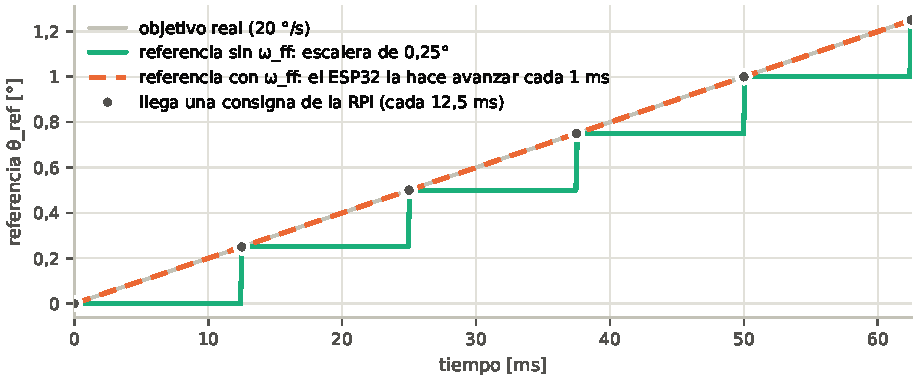
\includegraphics[width=0.95\linewidth]{ff_extrapolacion.pdf}
\caption{Referencia que ve el PI del ESP32 para un objetivo a $20\gr$/s. Si la RPi dejara de mandar consignas,
la extrapolación se detiene a los 50~ms; a los 100~ms actúa el \emph{watchdog} y el ESP32 retiene la posición.}
\label{fig:escalera}
\end{figure}

\textbf{Protecciones que siguen activas.} El feedforward no se salta ningún límite: la suma pasa por
$\omega_{\max}$ y por $\alpha_{\max}$, así que un salto de $\omega_{\mathrm{ff}}$ se convierte en una rampa. En los
límites de recorrido se anula. Y si el supervisor sale de SEGUIMIENTO, la RPi manda $\omega_{\mathrm{ff}} = 0$.

% ------------------------------------------------------------------------------------------
\section{Cuánto mejora}

\begin{figure}[H]
\centering
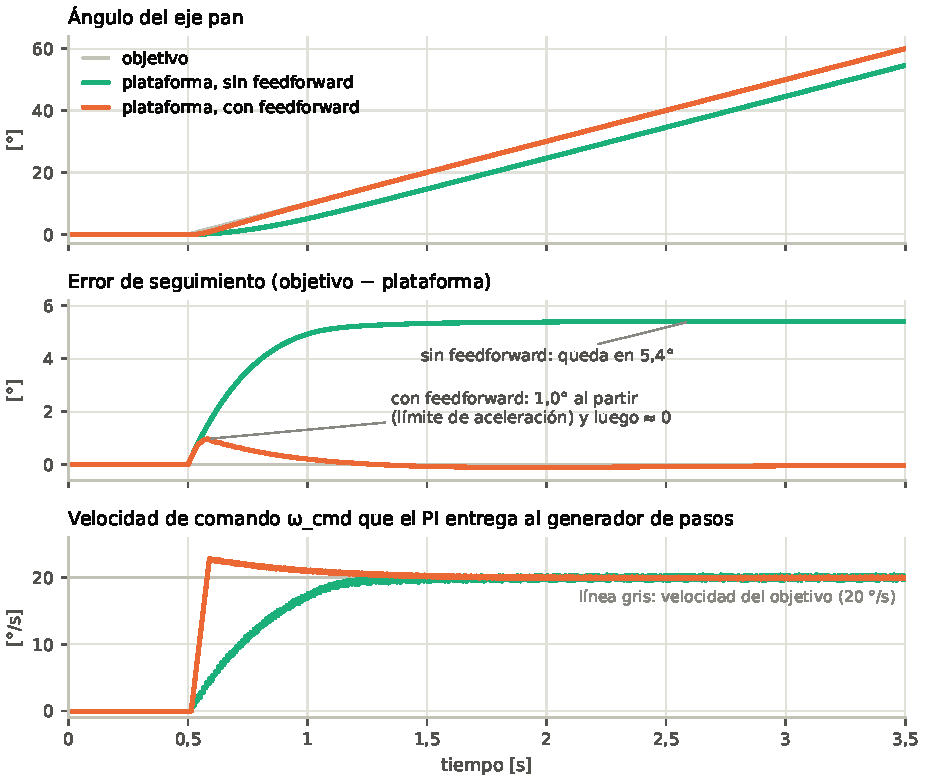
\includegraphics[width=0.97\linewidth]{ff_rampa.pdf}
\caption{Eje pan: el objetivo está quieto y en $t = 0{,}5$~s parte a $20\gr$/s. Lazo interno simulado con
consigna exacta cada 12,5~ms. Sin feedforward, la velocidad sale del error y el eje queda $5{,}4\gr$ atrás. Con
feedforward, el eje alcanza la velocidad en lo que permite la rampa de aceleración (67~ms) y el error vuelve a cero.}
\label{fig:rampa}
\end{figure}

\begin{figure}[H]
\centering
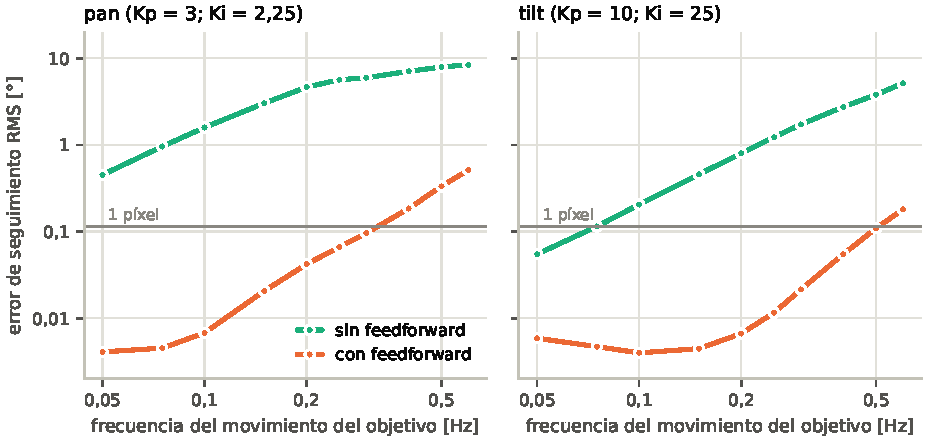
\includegraphics[width=\linewidth]{ff_frecuencia.pdf}
\caption{Objetivo que oscila con $15\gr$ de amplitud: error de seguimiento del lazo interno según la frecuencia.
Ejes logarítmicos. A 0,25~Hz la velocidad máxima es $24\gr$/s; a 0,5~Hz, $47\gr$/s.}
\label{fig:frec}
\end{figure}

\begin{table}[H]
\centering\small
\caption{Error de seguimiento RMS del lazo interno, objetivo senoidal de $15\gr$ (valores de la figura~\ref{fig:frec}).}
\begin{tabular}{@{}lcccccc@{}}
\toprule
 & \multicolumn{3}{c}{Pan} & \multicolumn{3}{c}{Tilt} \\
\cmidrule(lr){2-4}\cmidrule(l){5-7}
 & 0,1 Hz & 0,25 Hz & 0,5 Hz & 0,1 Hz & 0,25 Hz & 0,5 Hz \\
\midrule
Sin feedforward & $1{,}59\gr$ & $5{,}67\gr$ & $7{,}95\gr$ & $0{,}21\gr$ & $1{,}24\gr$ & $3{,}80\gr$ \\
Con feedforward & $0{,}007\gr$ & $0{,}07\gr$ & $0{,}33\gr$ & $0{,}004\gr$ & $0{,}012\gr$ & $0{,}11\gr$ \\
\bottomrule
\end{tabular}
\end{table}

Con el lazo completo (cámara, detector y predictor incluidos), la simulación de \cod{main.py} da lo mismo en
menor escala: el error de centrado en régimen baja de 28,6 a 2,3~px con orden 3 y $\lam = 0{,}80$
(\cod{docs/prediccion\_rls.pdf}, sección 5). El lazo completo mejora menos que el lazo interno porque ahí
$\omega_{\mathrm{ff}}$ ya no es exacta: viene del predictor, con su ruido y su atraso.

\textbf{Lo que el feedforward no arregla.} La aceleración. Con $\alpha_{\max} = 300\gr$/s$^2$, llegar a $20\gr$/s
toma 67~ms, y en ese rato se acumula cerca de $1\gr$ de error (figura~\ref{fig:rampa}). Por eso el error con
feedforward crece con la frecuencia en la figura~\ref{fig:frec}.

% ------------------------------------------------------------------------------------------
\section{Qué puede salir mal}

El PI se corrige solo: si ordena de más, el error cambia de signo y ordena de menos. El feedforward no: es una
orden directa, y lo que tenga de malo pasa al motor. La tabla~\ref{tab:sens} mide cuánto importa cada defecto.

\begin{table}[H]
\centering\small
\caption{Sensibilidad del feedforward. Eje pan, objetivo senoidal de $15\gr$ y 0,25~Hz; error RMS del lazo interno.}
\label{tab:sens}
\begin{tabular}{@{}llc@{}}
\toprule
Defecto de $\omega_{\mathrm{ff}}$ & Causa típica & Error RMS \\
\midrule
Ninguno (ideal) & & $0{,}07\gr$ \\
Ruido de $0{,}6\gr$/s & ruido de medición de $0{,}05\gr$ con $\lam = 0{,}80$ & $0{,}09\gr$ \\
Ruido de $1{,}8\gr$/s & ruido de medición de $0{,}15\gr$ & $0{,}18\gr$ \\
Atraso de 25 ms & & $0{,}29\gr$ \\
Atraso de 50 ms & $\lam$ alto: la velocidad estimada llega tarde & $0{,}51\gr$ \\
Atraso de 100 ms & & $0{,}96\gr$ \\
Escala 0,8 o 1,2 & micropasos o relación de transmisión mal configurados & $1{,}16\gr$ / $1{,}08\gr$ \\
Escala 0,5 & & $2{,}85\gr$ \\
\textbf{Sin feedforward} & & $\mathbf{5{,}67\gr}$ \\
Signo invertido & & $10{,}1\gr$ \\
\bottomrule
\end{tabular}
\end{table}

\begin{itemize}
  \item \textbf{El ruido importa poco.} El motor integra la velocidad, así que el ruido de $\omega_{\mathrm{ff}}$
        se promedia. Con el ruido esperado el error casi no cambia.
  \item \textbf{El atraso importa más.} Es otro motivo para no subir $\lam$: con 0,95 la memoria del predictor es
        de 250~ms y la velocidad que entrega es vieja.
  \item \textbf{La escala es lo más delicado.} $\omega_{\mathrm{ff}}$ viaja en grados por segundo del eje, y el
        firmware la convierte a pasos con los micropasos configurados (comando \cod{m}). Si ese valor no coincide
        con el del driver, el eje gira a otra velocidad. Con el PI solo ese error pasa inadvertido, porque el lazo
        lo compensa; con feedforward se ve de inmediato. Aun con un 20~\% de error de escala, el resultado es
        cinco veces mejor que sin feedforward.
  \item \textbf{El signo} no debería fallar: $\omega_{\mathrm{ff}}$ usa la misma convención que
        $\theta_{\mathrm{ref}}$. Si el eje sigue al objetivo sin feedforward, el signo está bien.
  \item \textbf{Los reinicios del predictor.} Mientras el estimador se rellena no hay velocidad, y la RPi manda
        $\omega_{\mathrm{ff}} = 0$ por dos o tres cuadros. Con feedforward activo eso se siente como un tirón; se
        resuelve con el reinicio informado propuesto para el gating.
  \item \textbf{La sincronía.} Si la pose del AS5600 se toma en un instante equivocado, parte del movimiento de la
        plataforma se confunde con movimiento del objetivo y entra a $\omega_{\mathrm{ff}}$. Con un error de 5~ms y
        la plataforma acelerando a $300\gr$/s$^2$ son $1{,}5\gr$/s: del orden del ruido, tolerable.
\end{itemize}

% ------------------------------------------------------------------------------------------
\section{Cómo activarlo y probarlo}

\begin{enumerate}
  \item \textbf{Confirmar la escala.} En la consola del ESP32: \cod{e 1} y luego \cod{t pan} y \cod{t tilt}. La
        prueba compara los grados ordenados con los que mide el sensor y avisa si los micropasos no coinciden.
  \item \textbf{Partir sin feedforward}, con el tablero abierto y \cod{--duracion 0}:\\
        \cod{python3 main.py --fuente camara --enlace trama --habilitar --monitor --duracion 0}
  \item \textbf{Mover el objetivo lento y parejo} (unos $10\gr$/s) y anotar el error de centrado del tablero. Sin
        feedforward debería verse un atraso proporcional a la velocidad, mayor en pan que en tilt.
  \item \textbf{Marcar la casilla ``Feedforward de velocidad''} sin detener el programa. El atraso debería caer.
        En el gráfico de $\omega_{\mathrm{cmd}}$ debería desaparecer el rizado.
  \item \textbf{Subir la velocidad del objetivo de a poco.} Si los motores suenan ásperos, subir $\lam$ a 0,85.
        Si el eje se adelanta o se atrasa de forma sostenida, la escala está mal: volver al paso 1.
  \item \textbf{Guardar el CSV} de una corrida con y otra sin feedforward. Las columnas \cod{wff\_pan},
        \cod{wff\_tilt}, \cod{dpan\_deg} y \cod{dtilt\_deg} permiten comparar con números.
\end{enumerate}

Alguien debe estar a cargo del corte durante la prueba: con feedforward la plataforma reacciona más rápido.

% ------------------------------------------------------------------------------------------
\section{En simple}

\begin{lamina}{Sin feedforward}
El motor sólo se entera de que el objetivo se movió cuando ya quedó atrás. Para seguirlo tiene que ir siempre un
poco atrasado, y mientras más rápido el objetivo, más atrasado.
\end{lamina}

\begin{lamina}{Con feedforward}
La cámara no sólo ve dónde está el objetivo: el predictor también calcula a qué velocidad va. Esa velocidad se le
entrega al motor directamente. El motor gira a la par del objetivo desde el principio, y el control de posición
queda sólo para corregir detalles.
\end{lamina}

\begin{lamina}{El costo}
El motor le cree a esa velocidad sin verificarla. Por eso tiene que estar bien calibrada, y por eso se mantienen
todos los límites de velocidad, aceleración y recorrido.
\end{lamina}

\end{document}
